\documentclass[a4paper, 12pt]{article}
\usepackage{titling}
\usepackage{array}
\usepackage{booktabs}
\usepackage{enumitem}
\usepackage{graphicx}
\usepackage{hyperref}
\usepackage{amssymb}
%\usepackage{mathtools}
\usepackage{listings}
\usepackage{amsmath}
\usepackage{color} %red, green, blue, yellow, cyan, magenta, black, white
\setlength{\heavyrulewidth}{1.5pt}
\setlength{\abovetopsep}{4pt}
\setlength{\parindent}{0pt}
\graphicspath{{.}}
\usepackage{float}
\usepackage[margin=1in]{geometry}
\definecolor{mygreen}{RGB}{28,172,0} % color values Red, Green, Blue
\definecolor{mylilas}{RGB}{170,55,241}
% Must be after geometry
\usepackage{fancyhdr}
\pagestyle{fancy}
\fancyhf{}
\rhead{NN Homework 5}
\lhead{P.Lukin, E. Ovchinnikova}
\cfoot{\thepage}

\setlength{\droptitle}{-5em}

\title{Neural Networks  \\
				- Homework 5 -}
\author{Petr Lukin, Evgeniya Ovchinnikova}
\date{Lecture date: 31 October 2016}

\begin{document}

%-------------------------------------------------------------------------------
\lstset{language=Matlab,%
    %basicstyle=\color{red},
    breaklines=true,%
    morekeywords={matlab2tikz},
    keywordstyle=\color{blue},%
    morekeywords=[2]{1}, keywordstyle=[2]{\color{black}},
    identifierstyle=\color{black},%
    stringstyle=\color{mylilas},
    commentstyle=\color{mygreen},%
    showstringspaces=false,%without this there will be a symbol in the places where there is a space
    numbers=left,%
    numberstyle={\tiny \color{black}},% size of the numbers
    numbersep=9pt, % this defines how far the numbers are from the text
    emph=[1]{break},emphstyle=[1]\color{red}, %some words to emphasise
    %emph=[2]{word1,word2}, emphstyle=[2]{style},
}

%-------------------------------------------------------------------------------

\maketitle

\section{Mind map}

\begin{figure}[h]
  \centering
  \caption{Mind map. Chapter 4 (first part) from Haykin’s book. A zoomed version is attached as MultilayerPerceptron.png \label{fig:MultilayerPerceptron}}
  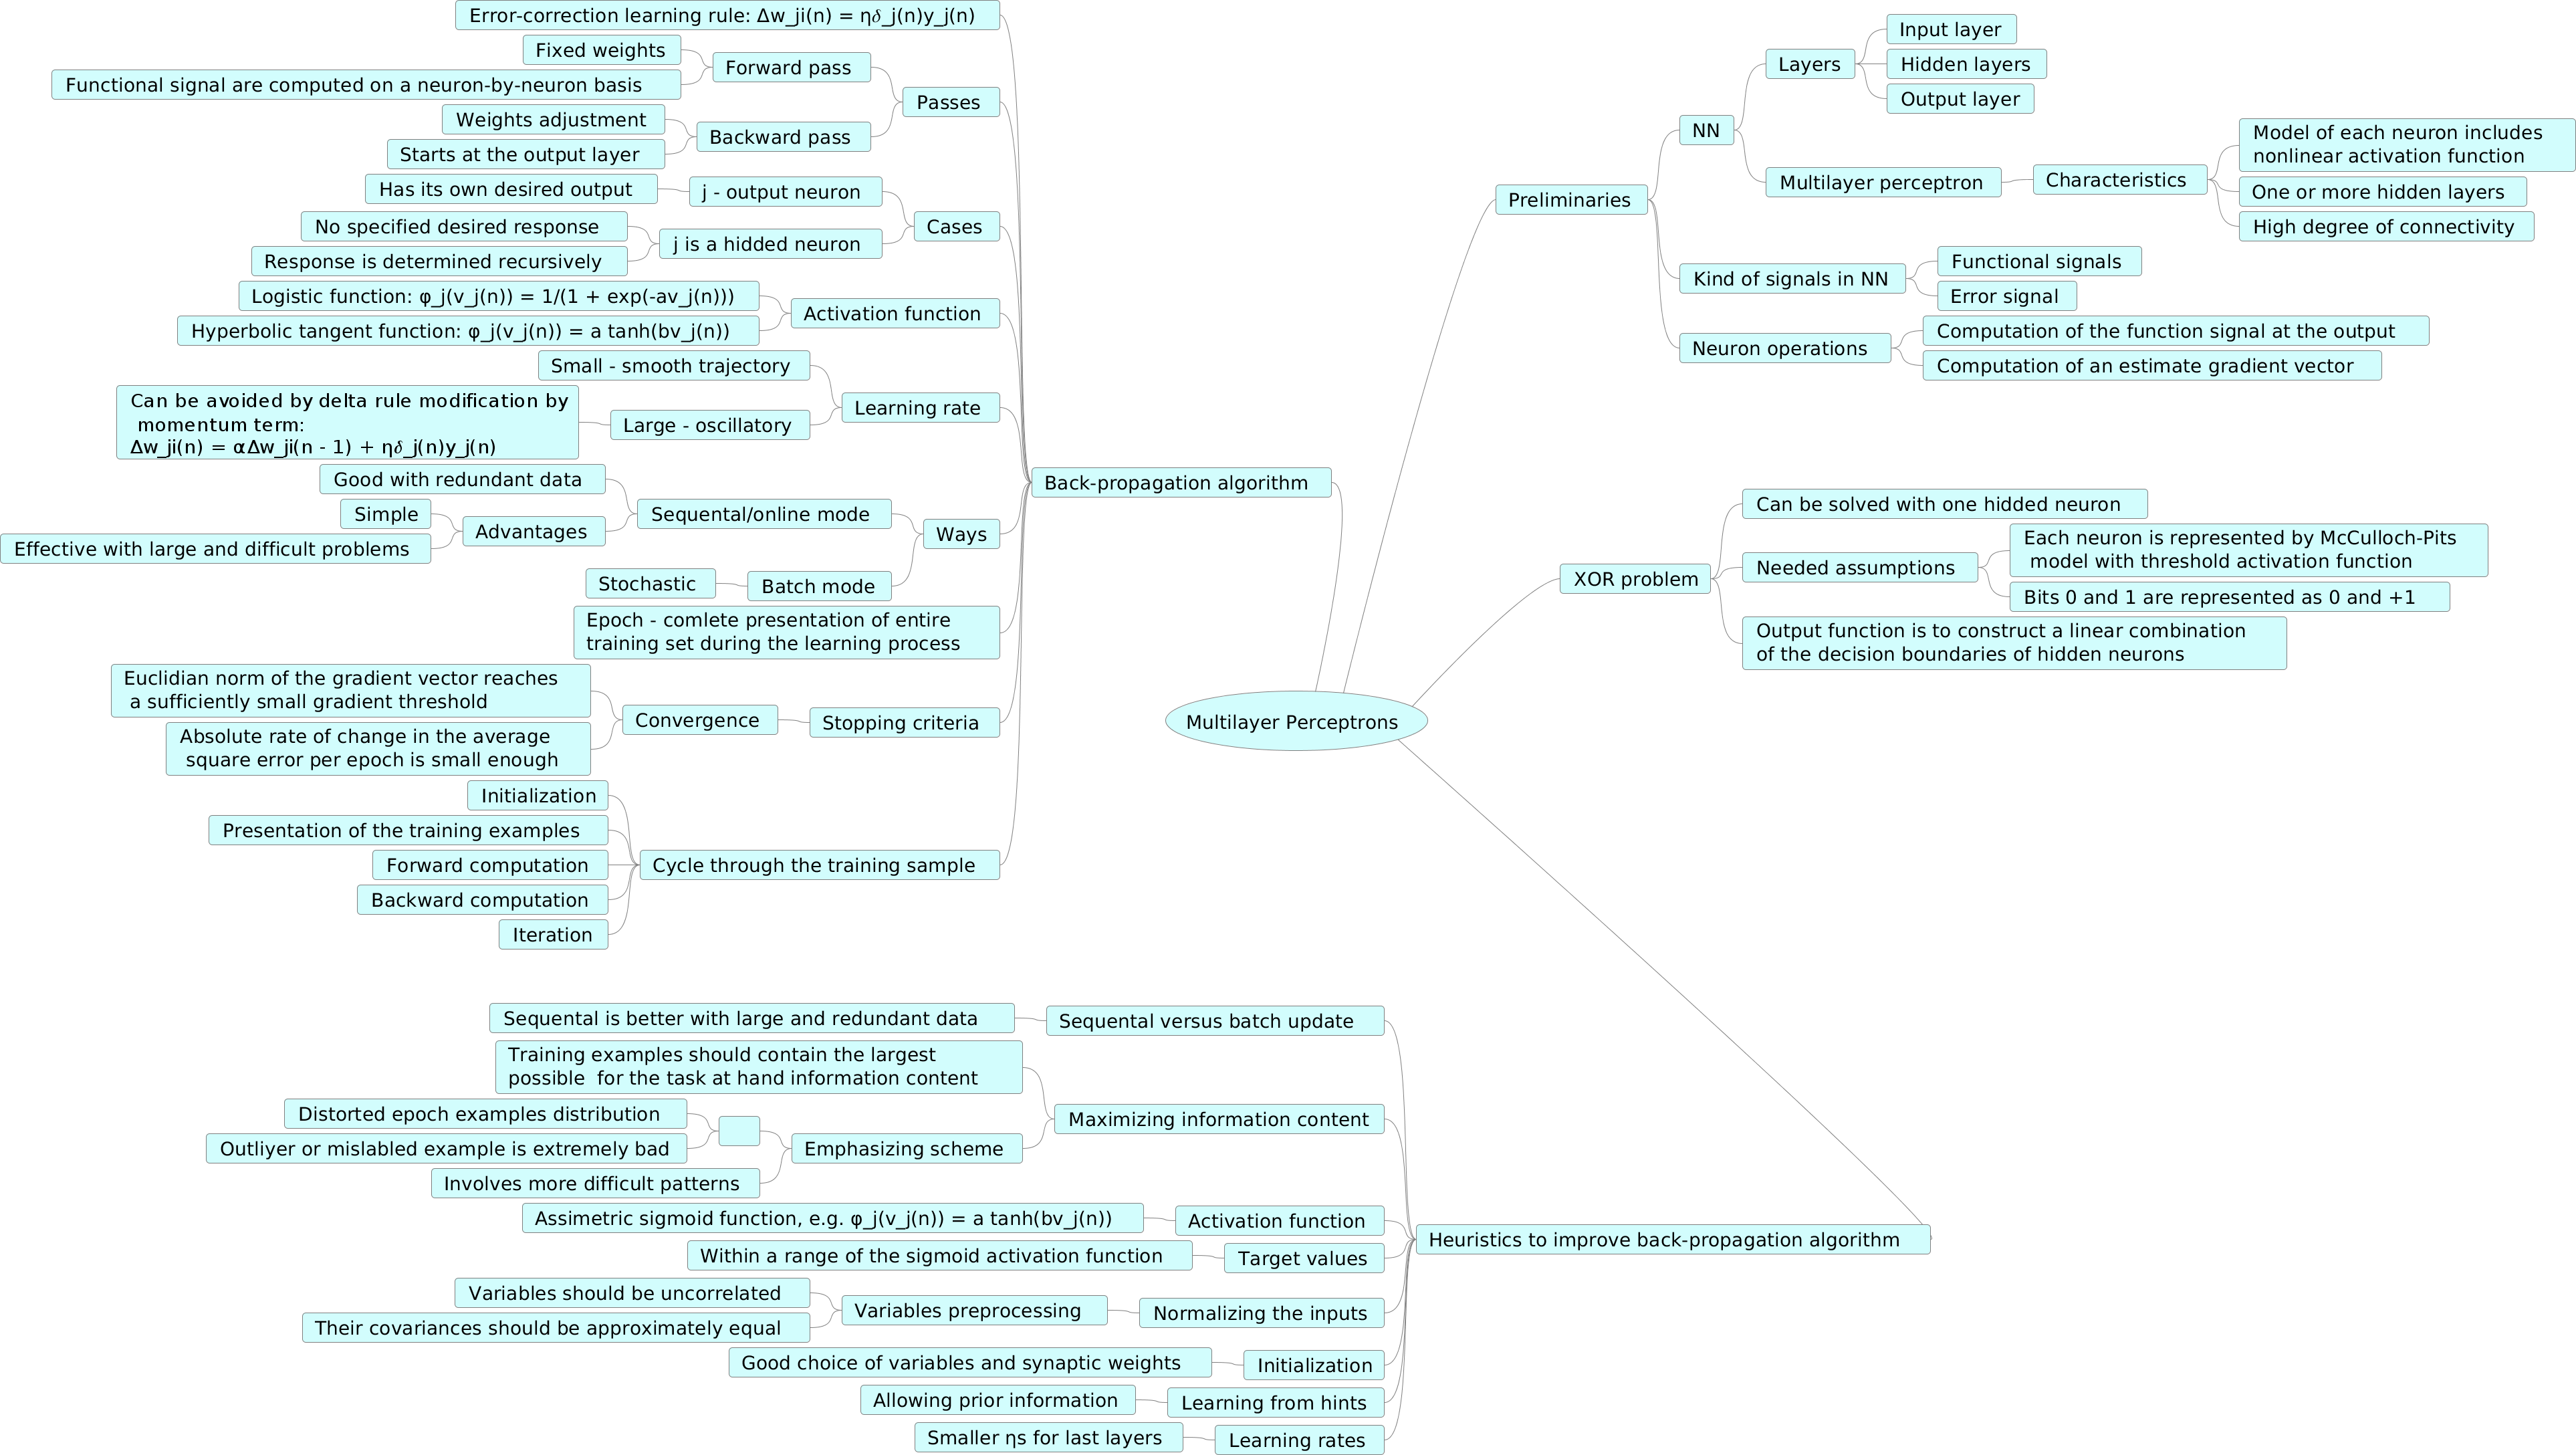
\includegraphics[width=1.1\textwidth]{MultilayerPerceptron}
\end{figure}

\section{Exercises}

\subsection{Exercise 2}

For this task you have to program the back-propogation (BP) for multi layered perceptron (MLP). Design your implementation for general NN with arbitrary many hidden layers. The test case is as follows:  2-2-1 multi layered perceptron (MLP) with sigmoid activation function on XOR data. \\

a. Experiments with initial weights\\

i. Train the network with zero initial weights i.e. $w_{ij}$ = 0.\\

ii. Train with random initial weights\\

Compare and comment on the convergence.\\

b. Experiment with different learning rates e.g. 0.1, 0.3, 0.5, 0.9.\\

Compare the convergence and plot some resulting surfaces. You are not allowed to use any neural network toolbox for this solution.\\

NB: If you fail to implement the general case in order to get the full points it is sufficient to implement only the use case (2-2-1 MLP)\\

\lstset{language=Python}
\begin{lstlisting}[frame=single]

\end{lstlisting}


\end{document}
